\documentclass{standalone}
\usepackage{tikz}
\usepackage{ctex,siunitx}
\usepackage{tkz-euclide}
\usepackage{amsmath}
\usetikzlibrary{patterns, calc}
\usetikzlibrary {decorations.pathmorphing, decorations.pathreplacing, decorations.shapes,}
\begin{document}
\small
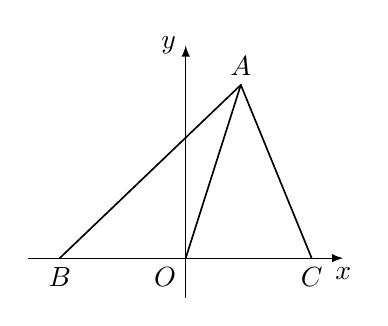
\begin{tikzpicture}[>=latex]
  \draw[thin,->](-2,0)--(2,0)node[below]{$x$};
  \draw[thin,->](0,-0.5)--(0,2.7)node[left]{$y$};
  \tkzDefPoints{0.7/2.2/A,-1.6/0/B,1.6/0/C,0/0/O}
  \tkzLabelPoints[below](B,C)
  \tkzLabelPoints[above](A)
  \tkzLabelPoints[below left](O)
  \tkzDrawSegments[semithick](A,B A,C A,O)
\end{tikzpicture}
\end{document}